%%%%%%%%%%%%%%%%%%%%%%%%%%%%%%%%%%%%%%%%%
% Dreuw & Deselaer's Poster
% LaTeX Template
% Version 1.0 (11/04/13)
%
% Created by:
% Philippe Dreuw and Thomas Deselaers
% http://www-i6.informatik.rwth-aachen.de/~dreuw/latexbeamerposter.php
%
% This template has been downloaded from:
% http://www.LaTeXTemplates.com
%
% License:
% CC BY-NC-SA 3.0 (http://creativecommons.org/licenses/by-nc-sa/3.0/)
%
%%%%%%%%%%%%%%%%%%%%%%%%%%%%%%%%%%%%%%%%%

%----------------------------------------------------------------------------------------
%	PACKAGES AND OTHER DOCUMENT CONFIGURATIONS
%----------------------------------------------------------------------------------------

\documentclass[final,hyperref={pdfpagelabels=false}]{beamer}

%\usepackage{rldmsubmit,palatino}
\usepackage{graphicx}
\usepackage{color}
\usepackage{multicol}
\usepackage{pdfpages}
\usepackage{caption}
% graph path
%\graphicspath{ {/Users/shuping.ruan/Dropbox/rldm/pic/} }
%%---------- my command -------------%%
\newcommand{\pard[1]}{\frac{\partial}{\partial{#1}}}
\newcommand{\mean[1]}{\frac{1}{n}\sum_{i=1}^{#1}}
\newcommand{\defeq}{\vcentcolon=}
\newcommand{\eqdef}{=\vcentcolon}
\newcommand\independent{\protect\mathpalette{\protect\independenT}{\perp}}
\newcommand{\wh}{\widehat}
\newcommand{\itl}{\intercal}
\newcommand{\p}{\prime}
\newcommand{\bs}{ \boldsymbol}
\newcommand{\mb}{\mathbb}
\newcommand{\ml}{\mathcal}
\newcommand{\br}{\bar}
\newcommand{\txt}{\text}
\newcommand{\lt}{\left}
\newcommand{\rt}{\right}
\newcommand{\lv}{\lvert}
\newcommand{\rv}{\rvert}
\newcommand{\nlim}{\underset{n \to \infty}{\lim}}
\newcommand{\smb}{\begin{bmatrix}}
	\newcommand{\sme}{\end{bmatrix}}
\newcommand\indep{\protect\mathpalette{\protect\independenT}{\perp}}
\def\independenT#1#2{\mathrel{\rlap{$#1#2$}\mkern2mu{#1#2}}}
\newcommand{\tsgn}{\txt{sgn}}


%%-------- my package -------%%
\usepackage{epstopdf}
\usepackage{cite}
\usepackage{amsmath}
\usepackage{color}
\usepackage{graphicx}
\usepackage{verbatim}
%\usepackage{bbm}
%\usepackage{xfrac}
%\usepackage{dsfont}
\usepackage{amssymb}
\usepackage{verbatim}
\usepackage{mathtools}
\usepackage{resizegather}
\usepackage{xfrac}
\usepackage{amsthm}
\usepackage[ruled]{algorithm2e}
%\newtheorem{remark}{Remark}
%\newtheorem{lemma}{Lemma}
%\newtheorem{theorem}{Theorem}
%\newtheorem{corollary}{Corollary}
%\newtheorem{theorem}{Theorem}[section]
%\newtheorem{lemma}[theorem]{Lemma}
%\newtheorem{proposition}[theorem]{Proposition}
%\newtheorem{corollary}[theorem]{Corollary}
\renewcommand\qedsymbol{$\blacksquare$}

%%----------------------------------------------------------------------------%%
%%---------------------------- Import Packages -----------------------------%%
%%----------------------------------------------------------------------------%%


\usepackage{booktabs}  % professionally typeset tables
\usepackage{amsmath}
\usepackage{textcomp}  % better copyright sign, among other things
\usepackage{xcolor}
\usepackage{lipsum}    % filler text
\usepackage{subfig}    % composite figures

% original packages
\usepackage[orientation=portrait,size=a0,scale=1.4]{beamerposter} % Use the beamerposter package for laying out the poster with a portrait orientation and an a0 paper size

\usetheme{I6pd2} % Use the I6pd2 theme supplied with this template

\usepackage[english]{babel} % English language/hyphenation

\usepackage{amsmath,amsthm,amssymb,latexsym} % For including math equations, theorems, symbols, etc

%\usepackage{times}\usefonttheme{professionalfonts}  % Uncomment to use Times as the main font
%\usefonttheme[onlymath]{serif} % Uncomment to use a Serif font within math environments

\boldmath % Use bold for everything within the math environment

\usepackage{booktabs} % Top and bottom rules for tables

\graphicspath{{figures/}} % Location of the graphics files

\usecaptiontemplate{\small\structure{\insertcaptionname~\insertcaptionnumber: }\insertcaption} % A fix for figure numbering

%----------------------------------------------------------------------------------------
%	TITLE SECTION 
%----------------------------------------------------------------------------------------

\title{\huge Dynamic Treatment Regimes under Constraints} % Poster title

\author{Shuping Ruan} % Author(s)

\institute{Department of Statistics, North Carolina State University} % Institution(s)

%----------------------------------------------------------------------------------------
%	FOOTER TEXT
%----------------------------------------------------------------------------------------

\newcommand{\leftfoot}{} % Left footer text

\newcommand{\rightfoot}{} % Right footer text

%----------------------------------------------------------------------------------------

\begin{document}

\addtobeamertemplate{block end}{}{\vspace*{2ex}} % White space under blocks

\begin{frame}[t] % The whole poster is enclosed in one beamer frame

\begin{columns}[t] % The whole poster consists of two major columns, each of which can be subdivided further with another \begin{columns} block - the [t] argument aligns each column's content to the top

\begin{column}{.02\textwidth}\end{column} % Empty spacer column

\begin{column}{.465\textwidth} % The first column

%----------------------------------------------------------------------------------------
%	Overview
%----------------------------------------------------------------------------------------

\begin{block}{Overview}
	\begin{itemize}
		\item Dynamic treatment regimes (DTRs) are sequential decision making problems in precision medicine.
		\item Most of the current methods for constructing DTRs focus on optimizing a single utility function over a finite number of decision time points (finite horizon).
		\item However, clinical situations often, in practice, require considering the trade-off among multiple competing outcomes without a priori fixed end of follow-up point (infinite horizon). 
		\item  Hence, we develop a method of estimating constrained optimal dynamic treatment regimes in chronic diseases where patients are monitored and treated throughout their life. 
		\item  Our method is demonstrated through a simulated cancer trial dataset based on a chemotherapy mathematical model.
	\end{itemize}
\end{block}

%----------------------------------------------------------------------------------------
%	Dataset
%----------------------------------------------------------------------------------------
            
\begin{block}{Dataset}
\begin{itemize}
\item Observed data structure: 

$$\ml{D} = \lt\{  (\bs{S}^i_{0}, A^i_{0}, \bs{R}^i_{0} , \bs{S}^i_{1}, \cdots, 
\bs{S}^i_{T_i-1} , A^i_{T_i-1}, \bs{R}^i_{T_i-1}, \bs{S}^i_{T_i}) \rt\}_{i=1}^n$$
\begin{itemize}
 \item Assume $n$ i.i.d. trajectories, and the causal inference assumptions for identifiability of the causal effect of a regime
 \item $T \in \mb{N}$ : the total number of follow-up time steps for a patient
 \item $\bs{S}_{t} \in \bs{\ml{S}}$: the vector of a patient clinical information recorded up to time $t$, aka \textit{ state}. If a patient passed away, $\bs{S}_t = \bs{\emptyset}$, aka \textit{absorbing state}
 \item $A_{t} \in \ml{A}$ : the treatment assignment at time point $t$,  aka \textit{action}
 \item $\bs{R}_{t} \in \mb{R}^J$: the 
 \textit{reward} vector obtained after treatment $A_{t}$ is assigned
%Moreover, if a patient dies during the follow-up, say at decision point $t$, we set $\bs{S}_t = \bs{\emptyset}$, referred as the absorbing state in RL. Then, the patient's treatment assignment at time $t$ is $A_t=\emptyset$, and his/er length of follow-up $T = t$.	
\end{itemize}
\end{itemize}
\end{block}

\begin{block}{Values of regimes}
	\begin{itemize}
\item  A dynamic treatment regime, or \textit{policy}, $\pi : \bs{\ml{S}} \to \mathcal{A}$, is defined as a function which maps the support of the state variable to the set of the possible treatment assignments.
 \item The value function $\bs{V}^{\pi}(\bs{s}) \in \mb{R}^J$ of a state under a certain policy $\pi$ is defined as the expected total discounted rewards when the process begins in state $\bs{s}$ and all decisions are made according to policy $\pi$.  $$\bs{V}^{\pi}\lt(\bs{s}\rt) = \mb{E}_{\bs{s}}^{\pi} \sum_{t=0}^{\infty} \gamma^{t} \, \bs{r}(\bs{s}_t, a_t, \bs{s}_{t+1}),$$ where $\mb{E}_{\bs{s}}^{\pi}$ is the expectation when the initial state is $\bs{s}$ and a policy $\pi$ is followed. $\gamma$ is the discount factor.
 \item  The state-action value function $\bs{Q}^{\pi}(\bs{s}, a) \in \mb{R}^J$ under policy $\pi$, is defined similar but the first step takes action $a$. Equivalently, it can be expressed recursively via the bellman equation, $$\bs{Q}^{\pi}(\bs{s}, a) = \int_{\bs{s}^{\prime}\in\bs{\ml{S}}} p\lt(\bs{s}^{\prime} \mid \bs{s}, a\rt) \lt( \bs{R}\lt(\bs{s}, a, \bs{s}^{\prime}\rt) + \gamma \, \bs{V}^{\pi}(\bs{s}^{\prime}) \rt).$$ 
However, the transition model $\mb{P}$ is unknown in clinical cases, and optimal regimes must be learn from observed dataset.  
\item Hence, we adopt the least-squared policy evaluation method (LSQ)  with Gaussian radial basis functions to estimate the value a regime [1].
\end{itemize}
\end{block}

%----------------------------------------------------------------------------------------
%	Constrained optimal regimes
%----------------------------------------------------------------------------------------

\begin{block}{Infinite-stage constrained optimal regimes}
\begin{itemize}
\item Our goal is to use dataset observed over a finite length of time steps to construct a deterministic regime in the setting of infinite horizon constrained Markov decision process.
\begin{equation*}
\begin{gathered}
\max_{\pi \in \Pi}  \,\, V_1(\pi), \\ 
\text{\textbf{subject to}}  \,\, V_j({\pi}) \le \nu_{j-1},
\end{gathered}
\end{equation*}
where $\nu_{j-1}$, for $j = 2, \cdots, J$, are bounds on the constraints.
\item To search over a feasible policy space with
manageable computation complexity, a quadratic function is used for policy function approximation. 
\item Interior-point method is used for constrained optimization [2]. 
\item Our method is applied to a dataset simulated using a modified chemotherapy mathematical model, a system of ordinary differential equations (ODE), originally developed by Zhao et al [3].
\end{itemize}
\end{block}
\end{column} % End of the first column

\begin{column}{.03\textwidth}\end{column} % Empty spacer column
 
\begin{column}{.465\textwidth} % The second column

%----------------------------------------------------------------------------------------
%	RESULTS
%----------------------------------------------------------------------------------------

\begin{block}{Results}

\begin{itemize}
\item Pareto efficient frontier plot
\begin{figure}
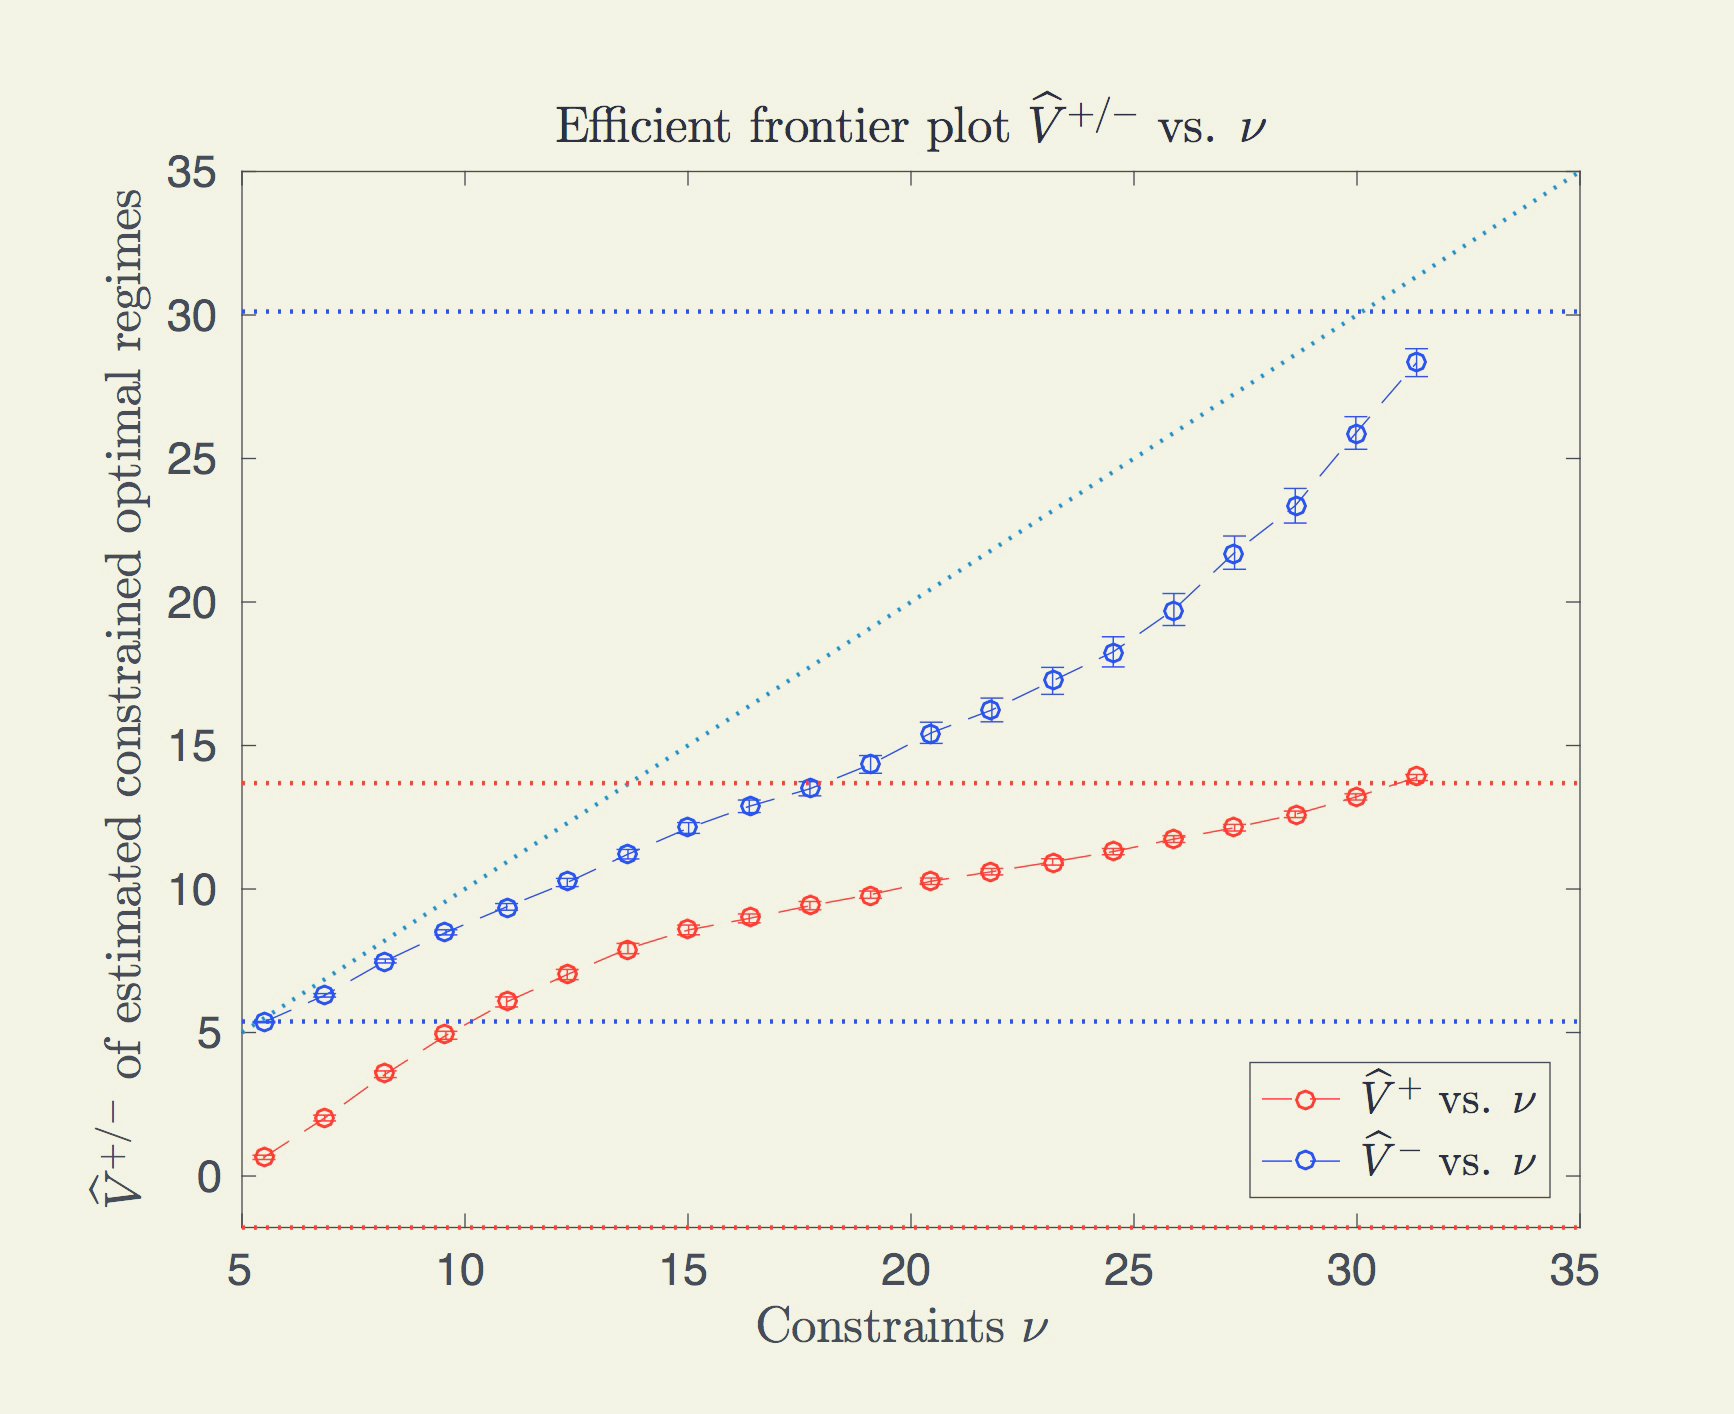
\includegraphics[width=0.7\linewidth]{efficient_plot.png}
\caption{Efficient frontier plot}
\end{figure}
\item Treatment
\begin{figure}
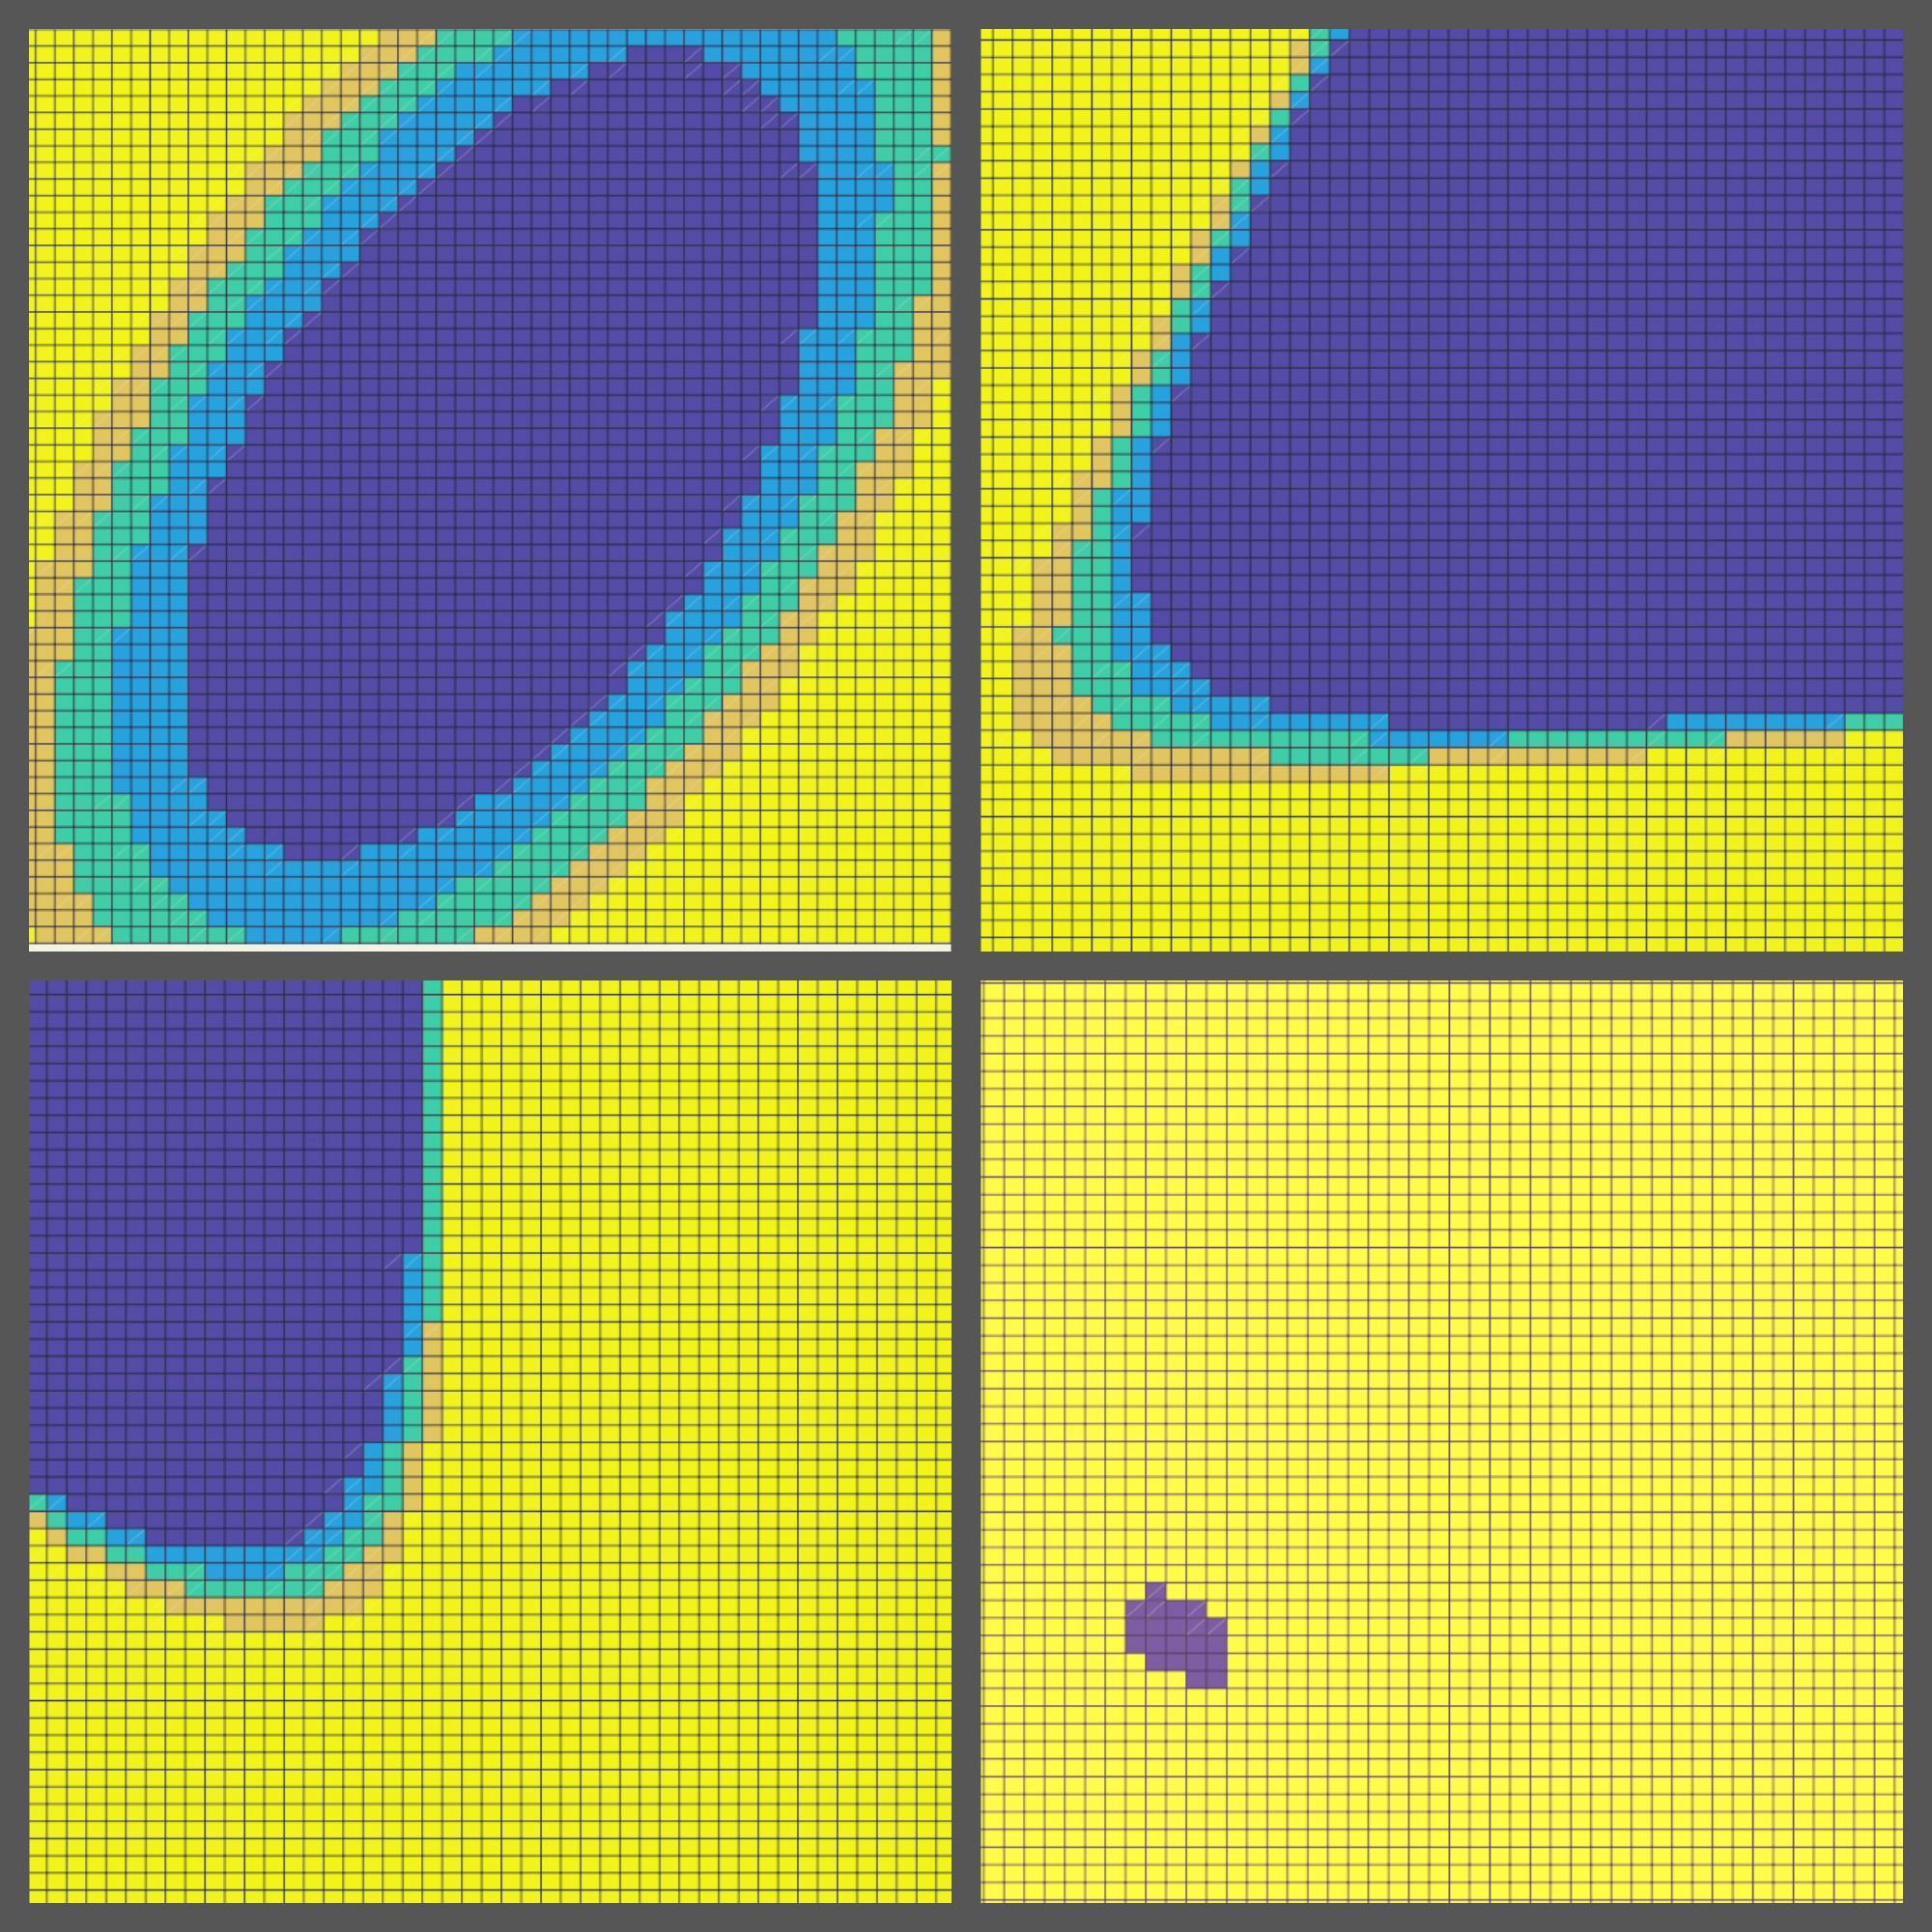
\includegraphics[width=0.5\linewidth]{act_dark.jpg}
\caption{Action for each state under a constraint bound. From left to right, up to botton, $\nu= 10, 17, 24, 31$. Yellow is a high dose treatment, and blue is low dose treatment.}
\end{figure}
\end{itemize}     
\end{block}


%----------------------------------------------------------------------------------------
%	CONCLUSION
%----------------------------------------------------------------------------------------

\begin{block}{Conclusion}

\begin{itemize}
\item We developed a method for constructing infinite-stage constrained optimal treatment regime using LSQ and interior point method.
\item Our method is suitable for batch off-line learning, due to the combination of LSQ and policy  approximation.
\item Our work is a foray to the practical use of dynamic treatment regimes in the real world applications, where handling multiple objectives in life-long clinical situation is inevitable.
\end{itemize}
\end{block}

%----------------------------------------------------------------------------------------
%	REFERENCES
%----------------------------------------------------------------------------------------

\begin{block}{References}
\nocite{*} % Insert publications even if they are not cited in the poster
\small{
	\bibliography{sample}
	\bibliographystyle{plain}
}
\end{block}

%----------------------------------------------------------------------------------------
%	ACKNOWLEDGEMENTS
%----------------------------------------------------------------------------------------

\begin{block}{Acknowledgments}

\begin{itemize}
\item I thank my advisor Dr. Eric Laber for his guidance.
\end{itemize}

\end{block}

%----------------------------------------------------------------------------------------
%	CONTACT INFORMATION
%----------------------------------------------------------------------------------------

\setbeamercolor{block title}{fg=black,bg=orange!70} % Change the block title color

\begin{block}{Contact Information}

\begin{itemize}
\item www.laber-labs.com
\item github.com/ShupingR
\item sruan@ncsu.edu
\item +1 (919) 348-3217
\end{itemize}

\end{block}

%----------------------------------------------------------------------------------------

\end{column} % End of the second column

\begin{column}{.015\textwidth}\end{column} % Empty spacer column

\end{columns} % End of all the columns in the poster

\end{frame} % End of the enclosing frame

\end{document}